\documentclass{standalone}
% Preamble
\begin{document}

  \section{Expérimentation}
  Nous choisissons $n=
\input{../txt/n.txt}
$ et le multidegré $
\input{../txt/deg.txt}
$.
La matrice de Bezout $B(1)$, à coefficients entiers, est de taille \input{../txt/Dx.txt} (figure de gauche). En permutant lignes et colonnes on obtient une matrice bloc-triangulaire supérieure (figure de droite) dont on peut calculer le noyau plus facilement.
On trouve que rang de $B(1)$ vaut \input{../txt/dim0.txt}. Une fois le processus de réduction terminé on obtient des matrices $B(1), B(x_j), j=1,\cdots,n$ de même taille, $B(1)$ étant inversible. La dimension du quotient $A$ est \input{../txt/dim.txt}. Les matrices compagnon $X_j = B(x_j)B(1)^{-1}$ fournissent les racines du système polynômial. On vérifie la qualité de chacune des racines obtenues en lui appliquant les polynômes $f_i, i=1,\cdots,n$. Les résultats sont représentés sous forme d'histogramme o\`u le logarithme décimal de l'erreur est porté en abscisse.
\begin{figure}[!ht]
  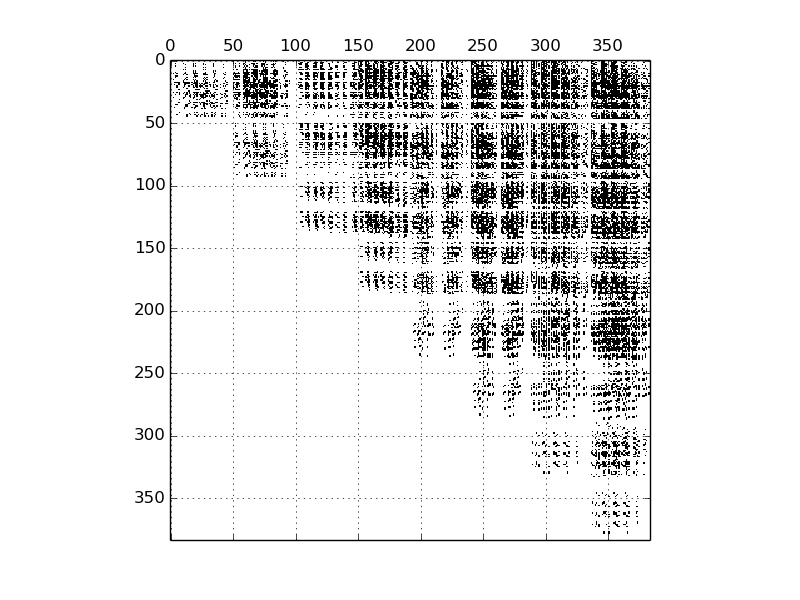
\includegraphics[height=8cm, width=1.2\textwidth]{../png/ref.png}
  \caption{histograms}
\end{figure}


Sur la figure de gauche nous avons les erreurs correspondants à l'algorithme o\`u le processus de réduction est effectué en arithmétique exacte (utilisant le logiciel Sage). Sur la figure de droite le processus de réduction est efféctué en arithmétique flottante (logiciel Octave).
Les temps de calcul en arithmétique flottante sont beaucoup plus rapides, mais au prix d'une dégradation sensible de la qualité des résultats.

\end{document}
